\documentclass[11pt]{article}
\usepackage{ctex}

\usepackage[left=1.25in,right=1.25in,top=1in,bottom=1in]{geometry}

% Copyright 20120 Liutao Tian, MIT License
% https://github.com/andy123t/code-latex-style/

\usepackage{listings,color}

% Matlab highlight color settings
%\definecolor{mBasic}{RGB}{248,248,242}       % default
\definecolor{mKeyword}{RGB}{0,0,255}          % bule
\definecolor{mString}{RGB}{160,32,240}        % purple
\definecolor{mComment}{RGB}{34,139,34}        % green
\definecolor{mBackground}{RGB}{245,245,245}   % lightgrey
\definecolor{mNumber}{RGB}{134,145,148}       % gray

\definecolor{Numberbg}{RGB}{237,240,241}     % lightgrey

% Python highlight color settings
%\definecolor{pBasic}{RGB}{248, 248, 242}     % default
\definecolor{pKeyword}{RGB}{228,0,128}        % magenta
\definecolor{pString}{RGB}{148,0,209}         % purple
\definecolor{pComment}{RGB}{117,113,94}       % gray
\definecolor{pIdentifier}{RGB}{166, 226, 46}  %
\definecolor{pBackground}{RGB}{245,245,245}   % lightgrey
\definecolor{pNumber}{RGB}{134,145,148}       % gray

\lstnewenvironment{Python}[1]{
	\lstset{language=python,               % choose the language of the code
		xleftmargin=30pt,
		xrightmargin=10pt,
		frame=l,
		framesep=15pt,%framerule=0pt,  % sets the frame style
		%frame=shadowbox,rulesepcolor=\color{red!20!green!20!blue!20},
		%basicstyle=\small\ttfamily,          % sets font style for the code
		basicstyle=\footnotesize\fontspec{Consolas},
		keywordstyle=\color{pKeyword},       % sets color for keywords
		stringstyle=\color{pString},         % sets color for strings
		commentstyle=\color{pComment},       % sets color for comments
		backgroundcolor=\color{pBackground}, % choose the background color
		title=#1,                            %\lstname show the filename of files
		emph={format_string,eff_ana_bf,permute,eff_ana_btr},
		emphstyle=\color{pIdentifier}
		showspaces=false,                    % show spaces adding particular underscores
		showstringspaces=false,              % underline spaces within strings
		showtabs=false,                      % show tabs within strings adding particular underscores
		tabsize=4,                           % sets default tabsize to 2 spaces
		captionpos=t,                        % sets the caption-position to bottom
		breaklines=true,                     % sets automatic line breaking
		framexleftmargin=5pt,
		fillcolor=\color{Numberbg},
		rulecolor=\color{Numberbg},
		numberstyle=\tiny\color{pNumber},
		numbersep=9pt,                      % how far the line-numbers are from the code
		numbers=left,                        % where to put the line-numbers
		stepnumber=1,                        % the step between two line-numbers.
}}{}

\lstnewenvironment{Python1}[1]{
\lstset{language=python,               % choose the language of the code
  xleftmargin=30pt,
  xrightmargin=10pt,
  frame=l,
  framesep=15pt,%framerule=0pt,  % sets the frame style
  %frame=shadowbox,rulesepcolor=\color{red!20!green!20!blue!20},
  %basicstyle=\small\ttfamily,          % sets font style for the code
  basicstyle=\footnotesize\fontspec{Consolas},
  keywordstyle=\color{pKeyword},       % sets color for keywords
  stringstyle=\color{pString},         % sets color for strings
  commentstyle=\color{pComment},       % sets color for comments
  backgroundcolor=\color{pBackground}, % choose the background color
  title=#1,                            %\lstname show the filename of files
  emph={format_string,eff_ana_bf,permute,eff_ana_btr},
  emphstyle=\color{pIdentifier}
  showspaces=false,                    % show spaces adding particular underscores
  showstringspaces=false,              % underline spaces within strings
  showtabs=false,                      % show tabs within strings adding particular underscores
  tabsize=4,                           % sets default tabsize to 2 spaces
  captionpos=t,                        % sets the caption-position to bottom
  breaklines=true,                     % sets automatic line breaking
  framexleftmargin=5pt,
  fillcolor=\color{Numberbg},
  rulecolor=\color{Numberbg},
  numberstyle=\tiny\color{pNumber},
  numbersep=9pt,                      % how far the line-numbers are from the code
  numbers=left,                        % where to put the line-numbers
  stepnumber=1,                        % the step between two line-numbers.
}}{}



\usepackage{graphicx}
\graphicspath{{figures/}}

\usepackage{fontspec}  % for Consolas
\usepackage{float}

\begin{document}
\section{shape}
矩阵的shape属性可以获得矩阵的形状。
\begin{Python}{获得的是一个元组}
import numpy as np

x = np.array([[0,1,2,3],[3,4,5,6],[6,7,8,9],[9,10,11,12],[12,13,14,15],[15,16,17,18],[18,19,20,21]])
#输出数组的行和列
print(x.shape)      #OUTPUT:(7,4)
#只输出行数
print(x.shape[0])
print(x.shape[-2])  #OUTPUT:7
#只输出列数
print(x.shape[1])
print(x.shape[-1])  #OUTPUT:4
\end{Python}
\section{numpy.sin}
numpy.sin(x, out=None, where=True, casting='same\_kind', order='K', dtype=None, subok=True)
\begin{Python}{画sin}
import numpy as np
import matplotlib.pylab as plt

x = np.linspace(-np.pi, np.pi, 201)
plt.plot(x, np.sin(x))
plt.xlabel('Angle [rad]')
plt.ylabel('sin(x)')
plt.axis('tight')
plt.show()
\end{Python}
\section{numpy.cos}
numpy.cos(x, /, out=None, *, where=True, casting='same\_kind', order='K', dtype=None, subok=True)
\begin{Python}{画cos}
	import numpy as np
	import matplotlib.pylab as plt
	
	x = np.linspace(-np.pi, np.pi, 201)
	plt.plot(x, np.cos(x))
	plt.xlabel('Angle [rad]')
	plt.ylabel('sin(x)')
	plt.axis('tight')
	plt.show()
\end{Python}




\section{numpy.mat}
将输入解释为矩阵。与矩阵不同,如果输入已经是矩阵或 ndarray,asmatrix 不会复制。
\begin{Python}{形式转换}
import numpy as np

x = np.mat('1.24125134 2; 3 4',dtype=np.float16)
print(x)
#   [[1.241 2.   ]
#    [3.    4.   ]]
\end{Python}
\section{numpy.array}
创建数组。nampy.array(object, dtype=None, copy=Ture, order='K', subok=False, admin=0, like=None)。

变量:

1.object:输入一个数组或序列。

2.dtype:数组所需的数据类型。如果没有给出,那么类型将被确定为在序列中保存对象所需的最小类型。

3.copy:如果为 true(默认),则复制对象。

4.order{'K','A','C','F'}:指定数组的内存布局。
K为内存中的顺序,A为任意顺序,C为按行顺序,F为按列顺序。

5.subok:如果为 True,则子类将被传递,否则返回的数组将被强制为基类数组(默认为False)。

6.ndmin:指定结果数组应具有的最小维数。将根据需要预先设置形状以满足此要求。

7.like:允许创建不是 NumPy 数组的数组的引用对象。

如果作为like传入的类数组支持\_\_array\_function\_\_协议,则结果由它定义。
在这种情况下,它确保创建一个与通过此参数传入的数组对象兼容的数组对象。
\begin{Python}{生成数组}
import numpy as np

a1 = np.array([1, 2, 3])
print(a1,id(a1))
#   [1 2 3] 2351076094192
a2 = np.array([[1, 2], [3, 4]])
print(a2)
#   [[1 2]
#    [3 4]]
b1 = np.array([1, 2, 3], dtype=complex)
#数据类型
#   bool:布尔类型
#   str :字符类型
#   int、uint:    有符号和无符号的32位整型
#   int8、uint8:  有符号和无符号的8位整型
#   int16、uint16:有符号和无符号的16位整型
#   int32、uint32:有符号和无符号的32位整型
#   int64、uint64:有符号和无符号的64位整型
#   float、float64:双精度浮点数
#   float32: 单精度浮点数
#   float16: 半精度浮点数
#   complex、complex128: 128位复数
#   complex64:    64位复数
print(b1)
#   [1.+0.j 2.+0.j 3.+0.j]
b2 = np.array([1, 2, 3], dtype=np.float32)
print(b2)
#   [1. 2. 3.]
d1 = np.array([(1,2),(3,4)],dtype=[('a','<U10'),('b','<U10')])
print(d1['a'])
#   ['1' '3']
print(d1['b'])
#   ['2' '4']
d2 = np.array([(1,2),(3,4)],dtype=[('a','<i4'),('b','<i4')])
print(d2['a'])
#   [1 3]
print(d2['b'])
#   [2 4]
c1 = np.array(a1, copy=True)
#print(c1,id(c1))
#   [1 2 3] 2351117108688
c2 = np.array(a1, copy=False)   #注意存储地址位置
print(c2,id(c2))
#   [1 2 3] 2351076094192
e1 = np.array([2, 3, 4, 1, 2, 5, 6, 0],order='K')
print(e1)
#   [2 3 4 1 5 6 0]
e2 = np.array([2, 3, 4, 5, 2, 5, 6, 0],order='A')
print(e2)
#   [2 3 4 5 2 5 6 0]
e3 = np.array([2, 3, 4, 1, 2, 6, 6, 0],order='C')
print(e3)
#   [2 3 4 1 2 6 6 0]
e4 = np.array([2, 3, 4, 1, 2, 5, 6, 9],order='F')
print(e4)
#   [2 3 4 1 2 5 6 9]
f1 = np.array(np.mat('1 2; 3 4'))
print(type(f1))
#   <class 'numpy.ndarray'>
f2 = np.array(np.mat('1 2; 3 4'),subok=True)
print(type(f2))
#   <class 'numpy.matrix'>
g1 = np.array([1, 2, 3], ndmin=3,)
print(g1)
#   [[[1 2 3]]]
\end{Python}
\section{numpy.percentile}
numpy.percentile(a, q, axis=None, out=None, overwrite\_input=False, interpolation='linear', keepdims=False)计算沿指定轴的数据的第q个百分位数。

a : array,用来算分位数的对象,可以是多维的数组

q : 介于0-100的float,用来计算是几分位的参数,如四分之一位就是25,如要算两个位置的数就(25,75)

axis : 坐标轴的方向,一维的就不用考虑了,多维的就用这个调整计算的维度方向,取值范围0/1

out : 输出数据的存放对象,参数要与预期输出有相同的形状和缓冲区长度

overwrite\_input : bool,默认False,为True时及计算直接在数组内存计算,计算后原数组无法保存

interpolation : 取值范围{'linear', 'lower', 'higher', 'midpoint', 'nearest'}
默认liner,比如取中位数,但是中位数有两个数字6和7,选不同参数来调整输出

keepdims : bool,默认False,为真时取中位数的那个轴将保留在结果中

\begin{Python}{百分位数}
import numpy as np

a = np.array([[10, 7, 4],[3, 2, 1]])
print(a)
#   [[10  7  4]
#    [ 3  2  1]]

b1 = np.percentile(a, 50)
b2 = np.percentile(a, (25, 75))
print(b1)
#   3.5
print(b2)
#	[2.25 6.25]

c = np.percentile(a, 50, axis=0)
d = np.percentile(a, 50, axis=1)
print(c)
#   [6.5 4.5 2.5]
print(d)
#   [7. 2.]

out = np.zeros_like(c)
g = np.percentile(a, 50, axis=0, out=out)
print(g)
#   [6.5 4.5 2.5]

e1 = a.copy()
print(e1)
#	[[10  7  4]
#	 [ 3  2  1]]
e2 = np.percentile(e1, 50, axis=1, overwrite_input=True)	#e1无法保存,节省内存
print(e2)
#	[7. 2.]
print(e1)
#	[[ 4  7 10]
#	 [ 1  2  3]]

a = np.array([2,9,9.8,0,11,12])		# 0, 2, 9, 9.8, 11, 12	
b0 = np.percentile(a, 50)
print(b0)   #9.4

b1 = np.percentile(a, 50, interpolation='linear')
print(b1)   #9.4

b2 = np.percentile(a, 50, interpolation='lower')
print(b2)   #9.0

b3 = np.percentile(a, 50, interpolation='higher')
print(b3)   #9.8

b4 = np.percentile(a, 50, interpolation='midpoint')
print(b4)   #9.4

b5 = np.percentile(a, 50, interpolation='nearest')
print(b5)   #9.0

f = np.percentile(a, 50, axis=1, keepdims=True)
print(f)
#   [[7.]
#    [2.]]
\end{Python}
\begin{Python}{percentile各个参数}
import matplotlib.pyplot as plt
import numpy as np

a = np.arange(4)
p = np.linspace(0, 100, 6001)
ax = plt.gca()
lines = [
('linear', None),
('higher', '--'),
('lower', '--'),
('nearest', '-.'),
('midpoint', '-.'),
]
for interpolation, style in lines:
ax.plot(
p, np.percentile(a, p, interpolation=interpolation),
label=interpolation, linestyle=style)
ax.set(
title='Interpolation methods for list: ' + str(a),
xlabel='Percentile',
ylabel='List item returned',
yticks=a)
ax.legend()
plt.show()
\end{Python}
\begin{figure}[H]
	\centering
	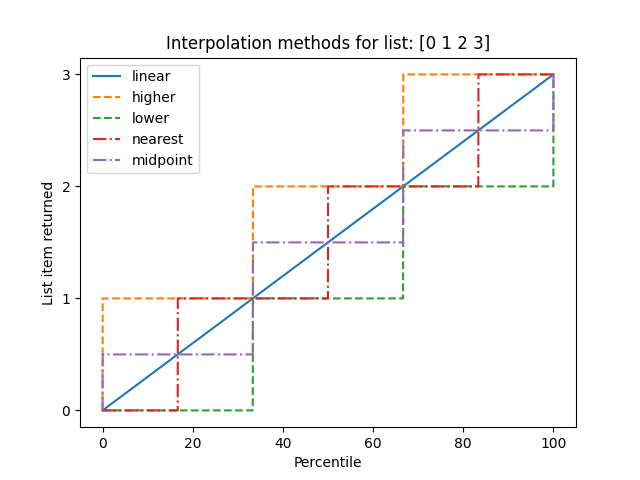
\includegraphics[scale=0.4]{percentile}
\end{figure}
\section{numpy.concatenate}
numpy提供了numpy.concatenate((a1,a2,...), axis=0)函数。能够一次完成多个数组的拼接。其中a1,a2,...是数组类型的参数,concatenate()效率更高,适合大规模的数据拼接。
\begin{Python}{数据的拼接}
import numpy as np

a1 = np.array([1,2,3])
b1 = np.array([11,22,33])
c1 = np.array([44,55,66])
d = np.concatenate((a1,b1,c1),axis=0)

a2 = np.array([[1,2,3],[4,5,6]])
b2 = np.array([[11,21,31],[7,8,9]])
e = np.concatenate((a2,b2),axis=0)		#第一个轴
f = np.concatenate((a2,b2),axis=1)		#第二个轴
g = np.concatenate((a2,b2),axis=-1)		#倒数第一个轴
h = np.concatenate((a2,b2),axis=-2)		#倒数第二个轴

print(d)
#OUTPUT:
#       [ 1  2  3 11 22 33 44 55 66]
print(e)
#OUTPUT:
#       [[ 1  2  3]
#        [ 4  5  6]
#        [11 21 31]
#        [ 7  8  9]]
print(f)
#OUTPUT:
#       [[ 1  2  3 11 21 31]
#        [ 4  5  6  7  8  9]]
print(g)
#OUTPUT:
#		[[ 1  2  3 11 21 31]
#		 [ 4  5  6  7  8  9]]
print(h)
#OUTPUT:
#		[[ 1  2  3]
#		 [ 4  5  6]
#		 [11 21 31]
#		 [ 7  8  9]]
\end{Python}
\section{numpy.dot}
两个数组的点积
\begin{Python}{数组点积}
import numpy as np

a = np.dot(3,4)
b = [[1, 0], [0, 1]]
c = [[4, 1], [2, 2]]

print(a)    
# 12
print(np.dot(b, c))
#
#  [[4 1]
#   [2 2]]
\end{Python}
\section{numpy.tile}
numpy.tile(A,reps)通过重复 A 由 reps 给出的次数来构造一个数组。reps是A 沿每个轴的重复次数。
\begin{Python}
	import numpy as np
	
	a = np.array([0,1,2])
	b = np.tile(a, 2)
	c = np.tile(a, (2,2))
	d = np.tile(a, (2,1,2))
	
	print(a)
	#   [0 1 2]
	print(b)
	#   [0 1 2 0 1 2]
	print(c)
	#   [[0 1 2 0 1 2]
	#    [0 1 2 0 1 2]]
	print(d)
	#   [[[0 1 2 0 1 2]]
	#
	#    [[0 1 2 0 1 2]]]
	
	a = np.array([[1,2],[3,4]])
	b = np.tile(a, 2)
	c = np.tile(a, (2,1))
	
	print(a)
	#       [[1 2]
	#        [3 4]]
	print(b)
	#       [[1 2 1 2]
	#        [3 4 3 4]]
	print(c)
	#       [[1 2]
	#        [3 4]
	#        [1 2]
	#        [3 4]]
	
	a = np.array([1,2,3,4])
	b = np.tile(a,(4,1))
	
	print(b)
	#       [[1 2 3 4]
	#        [1 2 3 4]
	#        [1 2 3 4]
	#        [1 2 3 4]]
\end{Python}
\section{numpy.clip}
numpy.clip(a, a\_min, a\_max, out=None, **kwargs),限制数组中的值。给定一个区间,区间外的值被剪裁到区间边缘。
\begin{Python}{限制数组中的值}
import numpy as np

a = np.arange(10)
print(a)
#[0 1 2 3 4 5 6 7 8 9]
b1 = np.clip(a, 1, 8)
print(b1)
#[1 1 2 3 4 5 6 7 8 8]
np.clip(a, 1, 8, out=b2)
print(b2)
#[1 1 2 3 4 5 6 7 8 8]
c = np.clip(a, 8, 1)
print(c)
#[1 1 1 1 1 1 1 1 1 1]
d = np.clip(a, [3, 4, 1, 1, 1, 4, 4, 4, 4, 4],8)
print(d)
#[3 4 2 3 4 5 6 7 8 8]



f = np.arange(10)
print(f)
#[0 1 2 3 4 5 6 7 8 9]
np.clip(a, 1, 8, out = f)	#out只能放回原始数组中
print(f)
#[1 1 2 3 4 5 6 7 8 8]
\end{Python}
\section{numpy.mean}
numpy.mean(a, axis=None, dtype=np.float64, out=None, keepdims=<no value>,where=<no value>)
计算沿指定轴的算术平均值。返回数组元素的平均值。
默认情况下,在扁平数组上取平均值,否则在指定轴上取平均值。 
dtype默认为float64中间值和返回值用于整数输入。
\begin{Python}{求平均值}
import numpy as np

a = np.array([[1,5,2],[3,4,2]])
b = np.mean(a, dtype=np.float32)
c = np.mean(a, where=[[True],[False]])
d = np.mean(a, axis=0)
f = np.mean(a, axis=1)
g = np.mean(a, keepdims=True)

print(a)
#OUTPUT:
#       [[1 5 2]
#        [3 4 2]]
print(b)
#OUTPUT: 2.8333333
print(c)
#OUTPUT: 2.6666667
print(d)
#OUTPUT: [2. 4.5 2.]
print(f)
#OUTPUT: [2.66666667 3.]
print(g)
#OUTPUT: [[2.83333333]]
\end{Python}
\section{numpy.random}
random随机函数
\subsection{numpy.random.normal}
random.normal(loc=0, scale=1, size=None)从正态(高斯)分布中抽取随机样本。

loc:为正态分布的中心。

scale:正态分布的标准偏差。

size:输出形状,如果给定的形状是,例如 (m, n, k),则抽取 m * n * k 个样本。如果size为None(默认),如果 loc和scale都是标量,则返回单个值。
\begin{Python}{正太分布}
import numpy as np

mean = 0,
variance = 1,
x = np.random.normal(loc = mean, scale= np.sqrt(variance), size=20)

unbiased_estimator = np.var(x, ddof=1)
biased_estimator = np.var(x, ddof=0)


print ("Unbiased_estimator : ",unbiased_estimator)
print ("Biased_estimator   : ", biased_estimator)

#OUTPUT:
#       Unbiased_estimator :  1.2392796506059365
#       Biased_estimator   :  1.1773156680756398
\end{Python}

\subsection{numpy.random.random()}
生成(0,1)以内的随机浮点数。也可以指定生成的个数,默认为1.
\begin{Python}{生成随机浮点数}
import numpy as np

attentuation1 = np.random.random()
attentuation2 = np.random.random((3,))
attentuation3 = 5 * np.random.random((3,2)) - 5     #前乘的数为了加大改变概率区间,原本区间为位于半开半闭区间[0, 1)之间的浮点数。

print(attentuation1)
print(attentuation2)
print(attentuation3)

#OUTPUT:
#       0.557983928722099
#
#       [0.46067162 0.66517044 0.68304871]
#
#       [[ 2.35169967 -0.70315046]
#        [-3.01499969  1.26146337]
#        [-3.42997838 -4.03027885]]
\end{Python}
\subsection{numpy.random.random\_sample()}
numpy模块中的np.random.random()和 np.random.random\_sample()函数生成的均是位于半开半闭区间[0, 1)之间的浮点数。
\begin{Python}{生成随机浮点数}
import numpy as np

attentuation1 = np.random.random_sample()
attentuation2 = np.random.random_sample((3,))
attentuation3 = 5 * np.random.random_sample((3,2)) - 5	#Three-by-two array of random numbers from [-5, 0)

print(attentuation1)
print(attentuation2)
print(attentuation3)

#OUTPUT:
#       0.25288115492026453
#
#       [0.9322892  0.20512729 0.98083572]
#
#       [[-1.96427089 -2.774898  ]
#        [-2.51141288 -2.0688131 ]
#        [-3.99685024 -0.38281138]]
\end{Python}
\subsection{numpy.random.rand()}
用法:numpy.random.rand(d0,d1,…,dn)

rand函数根据给定维度生成[0,1)之间的数据,包含0,不包含1。dn表示每个维度
返回值为指定维度的array
\begin{Python}{生成数据}
import numpy as np

a = np.random.rand(2,2)
b = np.random.rand(3)

print(a)
print('\n')
print(b)
#OUTPUT:
#       [[0.95641013 0.86736593]
#        [0.36199543 0.22519705]]

#       [0.63514646 0.62497891 0.87528597]
\end{Python}
\subsection{numpy.random.seed()}
np.random.seed()的作用:使得随机数据可预测。当我们设置相同的seed,每次生成的随机数相同。如果不设置seed,则每次会生成不同的随机数
\begin{Python}{随机数据可预测}
import numpy as np

np.random.seed(7)
a = np.random.rand(5)
np.random.seed(7)
b = np.random.rand(6)

print(a)
print(b)
#OUTPUT:
#       [0.07630829 0.77991879 0.43840923 0.72346518 0.97798951]
#       [0.07630829 0.77991879 0.43840923 0.72346518 0.97798951 0.53849587]
\end{Python}
\subsection{numpy.random.choice()}
numpy.random.choice(a, size=None, replace=True, p=None)
从给定的一维数组中生成随机数

参数: a为一维数组类似数据或整数;size为数组维度;p为数组中的数据出现的概率;当replace为False时,生成的随机数不能有重复的数值。
a为整数时,对应的一维数组为np.arange(a)

\begin{Python}{从指定数组生成随机数}
import numpy as np

a = np.random.choice(4)
b = np.random.choice(5, 3)
c = np.random.choice(5, 3, replace=False)
d = np.random.choice(5, size=(3,2))

demo_list = ['1', '4', '6', '3', '7', '2']
e = np.random.choice(demo_list,size=(2,4))
f = np.random.choice(demo_list,size=(2,4), p=[0.1,0.3,0.3,0.1,0.1,0.1])

print(a)
print('\n')
print(b)
print('\n')
print(c)
print('\n')
print(d)
print('\n')
print(e)
print('\n')
print(f)

#OUTPUT:
#2
#
# [0 2 2]
#
# [4 3 0]
#
# [[3 3]
#  [4 2]
#  [2 4]]
#
# [['3' '6' '3' '3']
#  ['2' '2' '4' '6']]
# 
# [['7' '4' '4' '7']
#  ['2' '1' '2' '2']]
\end{Python}
\subsection{numpy.random.uniform(low,high,size)}
功能:从一个均匀分布[low,high)中随机采样,注意定义域是左闭右开,即包含low,不包含high.

参数介绍:

low: 采样下界,float类型,默认值为0;

high: 采样上界,float类型,默认值为1;

size: 输出样本数目,为int或元组(tuple)类型,例如,size=(m,n,k), 则输出m*n*k个样本,缺省时输出1个值。

返回值:数组类型,其形状和参数size中描述一致。
\begin{Python}{size 为整数}
import numpy as np

s = np.random.uniform(0,1,5)
print(s)
#OUTPUT:
#       [0.56753576 0.40667623 0.10188742 0.3892323  0.51867366]
\end{Python}
\begin{Python}{size 为元组}
import numpy as np

s = np.random.uniform(0,1,[2,2])
print(s)
#OUTPUT:
#       [[0.9132833  0.06868765]
#        [0.62944324 0.07345442]]
\end{Python}

\section{其他}
\subsection{demo1}
X[n,:]是取第1维中下标为n的元素的所有值。

X[1,:]即取第一维中下标为1的元素的所有值。

X[:,  m:n],即取所有数据的第m到n-1列数据,含左不含右
\begin{Python}{数组的切块}
import numpy as np

X = np.array([[0,1],[2,3],[4,5],[6,7],[8,9],[10,11],[12,13],[14,15],[16,17],[18,19]])
Y = np.array([[0,1,2],[3,4,5],[6,7,8],[9,10,11],[12,13,14],[15,16,17],[18,19,20]])
print(X[:,0])

print(X[:,1])

print(X[1,:])

print(Y[:,1:3])

print(Y[...,:3])

print(Y[:3,2])

#OUTPUT:
#       [ 0  2  4  6  8 10 12 14 16 18]
#
#       [ 1  3  5  7  9 11 13 15 17 19]
#
# [2 3]
#
# [[ 1  2]
#  [ 4  5]
#  [ 7  8]
#  [10 11]
#  [13 14]
#  [16 17]
#  [19 20]]
#
#[[ 0  1  2]
# [ 3  4  5]
# [ 6  7  8]
# [ 9 10 11]
# [12 13 14]
# [15 16 17]
# [18 19 20]]
#
#[2 5 8]
\end{Python}
\subsection{demo2}
tf.matmul(A,C)=np.dot(A,C)= A@C都属于叉乘,而tf.multiply(A,C)= A*C=A∙C属于点乘
\begin{Python}{矩阵的运算}
import tensorflow as tf
import numpy as np

a = np.array([[1,2],[3,4]])
b = np.array([5,6])
c = np.array([[5,6],[7,8]])
print('a:'+'\n',a)
print('b:'+'\n',b)
print('c:'+'\n',c)
#叉乘
d1=a@c
d2=tf.matmul(a,c)
d3=np.dot(a,c)
#点乘
f1=a*c
f2=tf.multiply(a,c)

print('d1:叉乘a@c' + '\n', d1)
print('d2:叉乘matmul(a,c)' + '\n', d2)
print('d3:叉乘dot(a,c)' + '\n', d3)
print('f1:点乘a*c' + '\n', f1)
print('f2:点乘multiply(a,c)' + '\n', f2)

#OUTPUT:
#       d1:叉乘a@c
#           [[19 22]
#            [43 50]]
#       d2:叉乘matmul(a,c)
#           tf.Tensor(
#               [[19 22]
#                [43 50]], shape=(2, 2), dtype=int32)
#       d3:叉乘dot(a,c)
#           [[19 22]
#            [43 50]]
#       f1:点乘a*c
#           [[ 5 12]
#            [21 32]]
#       f2:点乘multiply(a,c)
#           tf.Tensor(
#               [[ 5 12]
#                [21 32]], shape=(2, 2), dtype=int32)
\end{Python}
\subsection{demo3}
一维数组切片跟list差不多 [Start:End:Step] 注意是不包含End。
\begin{Python}{一维切片}
import  numpy as np

a=np.array([1,2,3,4])
print(a[0:3:2])

#OUTPUT:
#		[1 3]
\end{Python}
二维数组切片。
\begin{Python}{二维切片}
import  numpy as np

a=np.array([[11,12,13,14],[21,22,23,24],[31,32,33,34],[41,42,43,44]])
print(a[0:4:2,0:4:2])

#OUTPUT:
#		[[11 13]
#		 [31 33]]
\end{Python}
None增加了一个维度.
\begin{Python}{None}
import numpy as np

a1 = np.array([1,2,3])
d = -a1[..., None]
f = -a1[..., None, :]

print(d)
print(f)

#OUTPUT:
#		[[-1]
#		 [-2]
#		 [-3]]
#
#		[[-1 -2 -3]]
\end{Python}
\subsection{demo4}
数据预处理
\begin{Python}{数据处理}
import os
import pandas as pd

os.makedirs(os.path.join('..', 'rpmnet1'), exist_ok=True)
data_file = os.path.join('..', 'rpmnet1', 'house_tiny.csv')
with open(data_file, 'w') as f:
f.write('NumRooms, Alley, Price\n')     #列名
f.write('NA,Pave,127500\n')
f.write('2,NA,10600\n')
f.write('4,NA,178100\n')
f.write('NA,NA,140000\n')

data = pd.read_csv(data_file)
print(data)

inputs, outputs = data.iloc[:, 0:2], data.iloc[:, 2]
inputs = inputs.fillna(inputs.mean())
print(inputs)

inputs = pd.get_dummies(inputs, dummy_na=True)
print(inputs)

import torch

x, y = torch.tensor(inputs.values, dtype=torch.float32), torch.tensor(outputs.values, dtype=torch.float32)
print(x)
print(y)
\end{Python}
\end{document}